\subsection{Cerrar sesión}

\begin{figure}[ht]
\centering
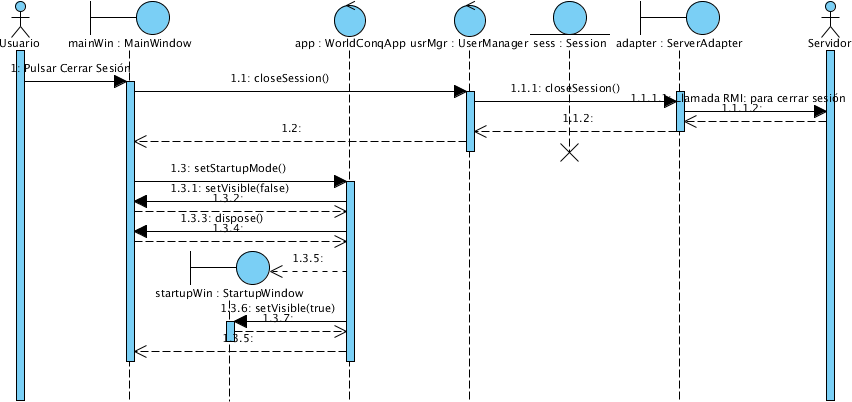
\includegraphics[scale=0.6]{img/ch03devel-logout.png}
\caption{Diagrama de secuencia de ``Cerrar sesión''}
\end{figure}

Estando en la ventana principal, el usuario puede decidir cerrar sesión en
cualquier momento. Este evento genera una llamada al gestor de usuarios. El
gestor de usuarios comunica al servidor que el usuario quiere cerrar la sesión.
Así mismo, destruirá la sesión que había hasta ahora.

A continuación se solicita a la clase \texttt{WorldConqApp} que vuelva a la
ventana de inicio realizando el paso inverso al detallado en la sección
anterior.
